%Análisis Experimental
%	Conjuntos de datos oficiales 
%	Criterios de la evaluación
%	Resultados 


\chapter{Análisis Experimental}
\label{cap:analisis}

En este capítulo se analiza la efectividad de la metodología de detección de sismos propuesta. 
%
Como parte de la preparación del experimento, la que se detalla en la sección \ref{sec:preparacionExperimento}, se definen los datos con los cuales se realiza la validación de los resultados (\textit{ground truth})  y se realiza un experimento base para identificar la configuración inicial óptima del algoritmo.


En la sección \ref{sec:evaluacion} se definen los criterios de evaluación de los resultados, que buscan replicar de la mejor forma posible la evaluación realizada en otros estudios del estado del arte y así obtener resultados comparables.
%
Luego se procede a evaluar los resultados obtenidos al utilizar diferentes conjuntos de atributos de interés\footnote{Revisar el capítulo \ref{cap:deteccion} para más detalles de la metodología de detección y los conceptos asociados.}.

Finalmente en la sección \ref{sec:conclusionEval} se discuten los resultados y la comparación con otros estudios. 

\section{Preparación del experimento}
\label{sec:preparacionExperimento}

Para evaluar la metodología propuesta se prepara un experimento que evalúa la efectividad de las detecciones a lo largo de un periodo de tiempo de 9 meses. A continuación se especifican los criterios de recolección utilizados y el periodo exacto a evaluar, así como también, los datos que se utilizaron como \textit{ground truth} en la evaluación de la detección en Chile e internacionalmente. 

Además se realiza un pequeño experimento, realizado sobre un subconjunto de los datos, para detectar los valores óptimos de configuración del algoritmo y que luego se utilizaron durante la evaluación completa que considera todos los datos.

Los datos utilizados para el experimento de configuración no están etiquetados manualmente, únicamente son el resultado del proceso de recolección que se detalla en la sección \ref{sec:recoleccion}.

	\subsection{Conjunto de datos de \textit{Twitter}}
	
		El flujo de datos $\mathcal{F}$ está conformado por \textit{tweets} publicados en \textit{Twitter} desde el 25 de Enero al 25 de Octubre del 2016 (9 meses). Técnicamente, sólo es posible acceder a una muestra del flujo público completo, por lo tanto, los datos son recuperados ya filtrados en base a palabras clave o atributos de interés especificados en $\mathcal{K}$ (en vez de obtener todo el flujo de datos y luego filtrar).  Para obtener los datos se utiliza la API para acceder al \textit{stream} público, tal como se explica en la sección \ref{sec:recoleccion} sobre recolección de datos. Los \textit{tweets} son procesados de manera estándar, normalizando el texto y removiendo duplicados (igual ID). El procesamiento es realizado considerando múltiples idiomas, incluyendo idiomas orientales, como chino, japonés, y persa. En total, el conjunto de datos utilizado para el análisis está compuesto por 53.557.475 \textit{tweets}.
		
		Los \textit{tweets} con coordenadas geográficas asociadas representan sólo el 8\% del conjunto de datos. La información geográfica fue incrementada mediante la incorporación de información de ubicación inferida, de forma similar a como lo hacen Robinson et al.~\cite{robinson2013sensitive}. Específicamente, se utiliza un índice geográfico para extraer nombres de localidades a partir del texto de los mensajes y de los perfiles de usuario. La extracción de datos se detalla en la sección \ref{sec:geocodificacion}. Utilizando este procedimiento, es posible geolocalizar el 53,6\% de la colección (28.723.948 \textit{tweets}).
		
	\subsection{Conjuntos de datos utilizados como \textit{Ground Truth}}
	
		Para verificar los resultados se utilizaron catálogos de sismos disponibles públicamente, uno correspondiente a una red de sensores global y otro a una red de sensores local. Se utilizaron las detecciones correspondientes al mismo periodo de 9 meses del conjunto de datos recolectados desde \textit{Twitter}. Ambos catálogos están constituidos por reportes oficiales y describen la localidad estimada del epicentro del sismo y la magnitud ~\cite{usgs:magnitude}.
		
\begin{description}
\item[Global (USGS):] 
		Catálogo construido por el \textit{Geological Survey} de Estados Unidos~\cite{usgs:data}. Este catálogo es muy completo para sismos de magnitud superior a $4.5$ ocurridos en diferentes partes del mundo ~\cite{earle2010omg}. Sin embargo, en el caso de sismos con magnitud inferior a $4.5$, los reportes consisten principalmente en eventos ocurridos en regiones específicas de Estados Unidos que tienen mejor cobertura de sensores. Para el periodo de estudio la USGS reportó 9.470 sismos con magnitud $\geq$ $4.0$ en todo el mundo. Se utilizó este conjunto de datos para evaluar el algoritmo propuesto y comparar su desempeño con otros sistemas que tienen cobertura mundial.

\item[Catálogo Local (GUC):]
		Este catálogo está focalizado en Chile y es generado por la Agencia Sismológica Nacional de Chile~\cite{guc:data}. Los reportes se basan en las detecciones realizadas por la extensa y densa red de sensores del GUC que es muy completa para sismos en Chile. Además de la información del epicentro y magnitud, este catálogo reporta la intensidad, indicando cuándo un sismo fue percibido por las personas y cuánto daño produjo (en la escala de intensidad modificada de Mercalli~\cite{usgs:mercalli}).
		Para el periodo de tiempo del estudio el GUC reportó 662 sismos de magnitud $\geq$ $4.0$, 476 de ellos clasificados como \textit{sismos sensibles}. Se utilizó este conjunto de datos para evaluar el algoritmo propuesto y comparar su desempeño con otros sistemas que tienen cobertura local. 
		
\end{description}
		
		Cabe destacar que durante el período de estudio, el GUC reportó 1.373 sismos en Chile ($\geq$ $3.6$) y el USGS reportó sólo 436 sismos en Chile con la misma magnitud (sólo 32\% de cobertura). Esto corrobora la necesidad de tener fuentes de información complementaria para completar la cobertura de sismos en áreas que no están del todo cubiertas por las redes de sismología globales o locales. 
		
	\subsection{Ajuste de parámetros iniciales óptimos}

	La metodología de detección de sismos propuesta requiere que se fijen 3 parámetros iniciales:
	\begin{enumerate}
		\item El umbral para detectar sismos $\theta$.
		\item La lista de atributos que definen un elemento de interés ($K$).
		\item El tamaño de la ventana de tiempo ($T$).
	\end{enumerate}
	
	A continuación se detalla cómo se determinaron los valores utilizados para realizar la configuración inicial del sistema. 

	\subsubsection*{1. Umbral para detectar sismos ($\theta$)}
	%
	Para determinar las variaciones significativas en el flujo $\mathcal{F}$ se identificó el valor óptimo para el umbral $\theta$ empíricamente. 
	%
	Utilizando una muestra de datos de 2 meses, se probó el sistema de detección usando diferentes valores de $\theta$ y se seleccionó el valor que maximiza el {\em F-measure}.
	%
	La tabla~\ref{table:zscore} muestra los resultados obtenidos y el valor seleccionado $\theta=1.5$.
	\begin{table}
\centering
\begin{tabular}{cccc}
\toprule
{z-score ($\theta$)} & {Precision} & {Recall} & {F-Measure} \\ 
\midrule
{0.5}    & {48.1\%}     & {79.9\%}  & {60.1\%}  \\ 
{1.0}    & {62.6\%}     & {65.0\%}  & {63.8\%}  \\ 
{\bf 1.5}    & {\bf 88.3\%}     & {\bf 54.2\%}  & {\bf 67.1\%}  \\
{2.0}    & {92.3\%}     & {29.0\%}  & {44.2\%}  \\ 
\bottomrule
\end{tabular}
\caption{Comportamiento del algoritmo utilizando diferentes valores para el umbral de detecci\'on de sismos $\theta$.}
\label{table:zscore}
\end{table}



	\subsubsection*{2. Listado de atributos que definen un elemento de interés ($K$)} 
	Como se mencionó previamente, en esta adaptación los elementos de interés ($K$) son una lista de palabras clave relacionadas con la ocurrencia de sismos.
	%
	En esta tesis se extendió la lista de palabras entregada por investigadores del USGS, que fue usada por Earle et al.~\cite{earle2012twitter} y Avvenuti et al.~	\cite{avvenuti2014earthquake,avvenuti2014ears}.
	%
	Sin embargo, a diferencia de los sistemas anteriores, la lista de palabras utilizada se construyó intentando incluir la mayor cantidad posible de palabras relacionadas con ocurrencias de sismos en cualquier idioma, incluso si incluía términos ambiguos (es decir, términos que a veces son utilizados en otros contextos).
	%
	Los mensajes ruidosos que puedan ser obtenidos al usar términos ambiguos no afectan el rendimiento de este método ya que es tolerante al ruido. 
	%
	Por ejemplo, la palabra ``quake'' puede ser usada para referirse a un videojuego o al personaje de un comic con el mismo nombre, o la palabra ``terremoto'' que en Chile también es utilizada para referirse a una bebida alcohólica típica y muy consumida durante las celebraciones nacionales. 
	%	
	La lista de palabras está compuesta por los términos listados en la figura \ref{img:keywords}. 
	%
	En caso de ser necesario modificar los términos de la lista, ésta puede ser actualizada dinámicamente.
	
	\begin{figure}[h!]
	\centering
	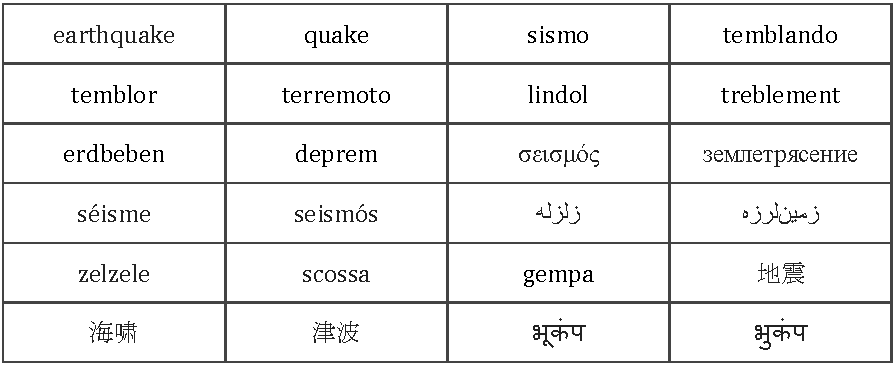
\includegraphics[width=0.8\textwidth]{imagenes/Keywords.pdf}
	\caption{Palabras clave utilizadas para recolectar \textit{tweets} relacionados con sismos.}
	\label{img:keywords}
	\end{figure}
	
	
	Además de las palabras clave relacionadas con sismos, se realizaron experimentos en los cuales además de las palabras clave, también se consideraban otros atributos para determinar si un elemento era de interés o no. 
	%
	De esta forma se pudo analizar la señal discreta asociada a diferentes tipos de atributos y determinar si estos agregaban valor a la detección o no. 
	%
	Entre estos atributos se encuentran:
	\begin{itemize}
	\item Sentimiento positivo del \textit{tweet}.
	\item Sentimiento negativo del \textit{tweet}.
	\item Idioma en el cual fue escrito el \textit{tweet}
	\item País mencionado en el texto del \textit{tweet}.
	\item País mencionado en la localidad de perfil del usuario que escribió el \textit{tweet}.
	\end{itemize}

	\subsubsection*{(3) Tamaño de la ventana de tiempo ($T$)} 
	El tamaño de la ventana corresponde al largo del tiempo (en segundos) de cada conjunto de \textit{tweets} en los cuales son divididos los datos de la entrada para ser procesados por el algoritmo.
	%
	Este parámetro se determina analizando el flujo de la entrada y seleccionando un valor para $T$ que minimiza la desviación estándar relativa, es decir, cuando la frecuencia de aparición es más estable. 
	%
	Intuitivamente, si la ventana de tiempo es muy pequeña, los mensajes que contengan elementos en $K$ estarán distribuidos de forma más aleatoria en cada ventana. 	
	%
	Esto significa que habrían ventanas de tiempo sin ninguna ocurrencia y otras con varias ocurrencias.
	%
	Mientras más grande sea la ventana de tiempo, más factible es poder estimar la frecuencia en la ventana siguiente. 
	%
	Para determinar el valor de $T$ se utilizó el siguiente procedimiento, descrito en~\cite{guzman2013line}:

	\begin{itemize}
	\item Para el flujo de entrada dado, se calcula la velocidad de llegada relativa de ventanas sucesivas $w_i$ de tamaño $T$.

	\item Se repite este proceso para diferentes tamaños de ventana $T$ en el rango de $0$ hasta $3\,600$ segundos (una hora) para un periodo de 2 meses y se selecciona el $T$ con la desviación estándar relativa más pequeña. En este caso el valor de tamaño de ventana que minimiza la desviación estándar corresponde a los valores para $T \geq 300$ segundos, tal como se muestra en la figura~\ref{fig:window_size}.

	\end{itemize}
	
	\begin{figure}[ht]
  	\centering
  	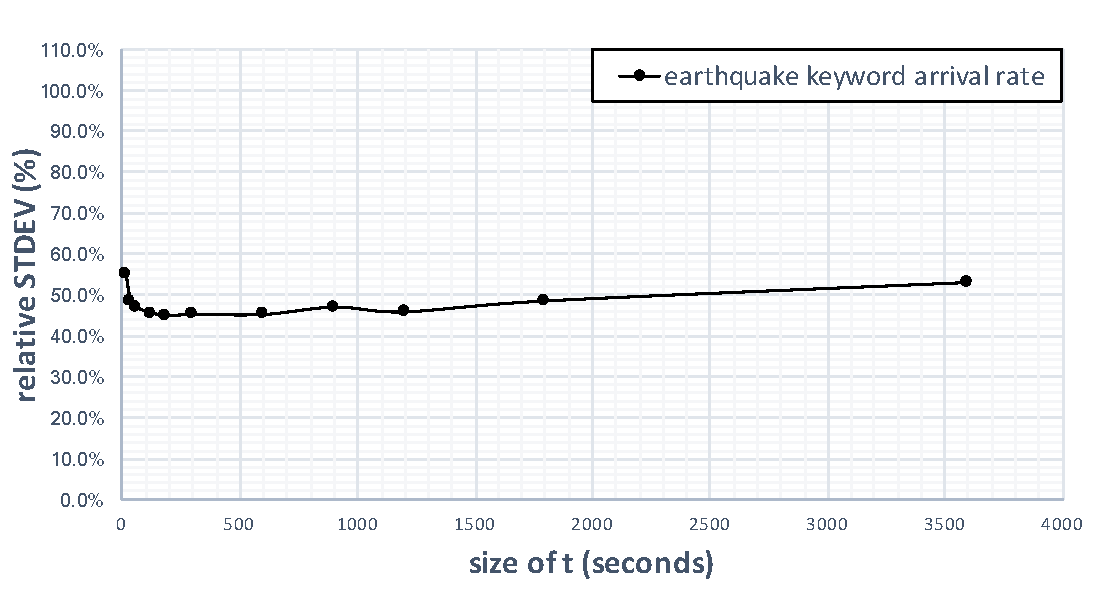
\includegraphics[trim={5 0 5 10}, clip, width=\textwidth]{imagenes/02_Poise_Analysis_WindowSize_solo.pdf}
  	\caption{Desviación estándar relativa de la señal que considera las palabras clave relacionadas con sismos para diferentes tamaños de ventana de tiempo (en segundos)}
	\label{fig:window_size}
	\end{figure}

	Además, para disminuir los tiempos de detección, el sistema ejecuta dos procesos paralelos idénticos desfasados en $150$ segundos uno del otro y con ello asegurar un tiempo de detección de máximo 5 minutos. 

		
\section{Evaluación}
\label{sec:evaluacion}

En esta sección se presenta la evaluación del método de detección de sismos propuesto. La evaluación se realizó utilizando 5 tipos de variaciones del flujo de entrada $\mathcal{F}$ creado a partir de mensajes que contienen palabras relacionadas con sismos $\mathcal{K}$. Estos 5 tipos de flujos son:

\begin{description}

\item[Palabras clave de sismos:] Señal que representa la velocidad de llegada relativa de los mensajes que contienen algún elemento en $\mathcal{K}$, donde $\mathcal{K}$ corresponde a la lista de palabras clave de sismos.
 
\item[Geolocalización a partir del texto:] Los \textit{tweets} seleccionados usando las palabras clave de sismos y que además mencionan algún país en el texto del \textit{tweet} son etiquetados utilizando el nombre de cada país. Estos \textit{tweets} son separados en distintos flujos de mensajes en base a las etiquetas, es decir, un flujo por cada país. Luego se calcula la velocidad de llegada relativa de los mensajes en cada flujo y la secuencia de velocidades relativas se analiza en forma de señal para detectar ráfagas.

\item[Geolocalización a partir del perfil del usuario:] Creado de manera similar a las señales de \textit{geolocalización a partir del texto}, con la diferencia que las etiquetas de localidades son extraídas desde el perfil del usuario.

\item[Idioma:] Creado de manera similar a las señales de \textit{geolocalización a partir del texto y del perfil del usuario}, con la diferencia que las etiquetas corresponden a los idiomas utilizados para escribir el texto del \textit{tweet}. Los diferentes flujos son analizados de la misma forma, generando señales representando la velocidad de llegada relativa de los mensajes. 

\item[Sentimiento:] Los \textit{tweets} seleccionados usando las palabras clave relacionadas con sismos son analizados para detectar si corresponden a un mensaje con sentimiento positivo o negativo. El análisis de sentimiento se describe con más detalle en la sección \ref{sec:sentimiento}. Los \textit{tweets} etiquetados se separan en dos flujos, un flujo con los mensajes con polaridad positiva y otro con los mensajes con polaridad negativa. Luego se analizan las señales generadas calculando la velocidad de llegada relativa de los \textit{tweets} que componen cada flujo.

\end{description}

\subsection{Metodología de evaluación}

La evaluación se realizó intentando satisfacer los criterios utilizados en los estudios que conforman el estado del arte con los cuales se desea comparar el sistema~\cite{sakaki2010earthquake,avvenuti2014ears,robinson2013sensitive,earle2012twitter}. Se replicaron los experimentos usando el conjuntos de datos de \textit{Twitter} descrito previamente y los datos utilizados como \textit{ground truth}, los cuales son equivalentes a los utilizados en las evaluaciones de otros estudios. Sin embargo no fue factible replicar los otros sistemas para compararlos utilizando exactamente los mismos datos. Esto se debe principalmente a que no tenemos acceso al código fuente, modelos ni detalles de implementación de esos sistemas. Debido a los altos costos asociados a los enfoques supervisados (es decir, etiquetado de datos y parametrización), que se describen en el capítulo \ref{cap:marco}. Por lo tanto, se reportan los resultados y luego se comparan de la forma más cercana posible a los resultados reportados por sistemas similares.

Hay algunas consideraciones relacionadas al uso de los catálogos de sismos utilizados como \textit{ground truth} en los sistemas basados en datos sociales:

\begin{enumerate}

\item  \textit{No todos los sismos en un catálogo fueron percibidos por las personas}. Por lo tanto, cualquier sistema que dependa de los \textit{sensores sociales o ciudadanos} puede potencialmente detectar sólo  un subconjunto de sismos que fueron efectivamente percibidos por humanos. Idealmente, un \textit{ground thruth} perfecto para sistemas basados en datos sociales debería considerar únicamente los sismos que fueron percibidos por personas. 

\item \textit{No todos los sismos en un catalogo que fueron sentidos por personas están etiquetados oficialmente como ``sismos sensibles''}. Esta discrepancia ocurre cuando las personas encargadas de reportar oficialmente la intensidad del sismo no advierten el suceso (principalmente durante sismos de baja intensidad). Idealmente, un \textit{ground truth} perfecto debería tener todos los sismos percibidos etiquetados como \textit{sismos sensibles}. 

\item \textit{Los catálogos de sismos con magnitud inferior a 4.0 de las agencias sismológicas no están siempre completas (no tienen \textit{recall} perfecto)}. Los reportes de sismos están basados en detecciones realizadas por múltiples sensores sismográficos que componen una red. Sin embargo, si un sismo ocurre en un área sin sismógrafos o con una baja densidad de sensores, estos no son reportados. Esto se refiere a la integridad el catálogo y también se discute en \cite{earle2010omg}. 
\end{enumerate}

\begin{table*}[!h]
\centering
\begin{tabular}{lcccc}
    \toprule
    \textbf{Trabajo}  & \textbf{Técnica} & \textbf{Cobertura} & \textbf{Palabras} & \textbf{Activo} \\ 
    \midrule
    Twicalli & No Supervisado & Mundial & \begin{tabular}[c]{@{}c@{}} earthquake, sismo, quake, \\temblor,
    temblando, gempa, \\lindol, tremblement, erdbeben, \\ deprem, seismós, séisme, \\ 
    zelzele, terremoto, scossa  \\ y traducciones de sismo en \\ Japonés, Chino, Griego \\ y Persa
    \end{tabular} & Si \\ 
    \midrule
    EARS & Supervisado & Italia  & scossa, terremoto & Si \\ 
    \midrule
    Sakaki et. al. & Supervisado & Japón  & earthquake, shaking & Si \\ 
    \midrule
    Earle et al. & No Supervisado & Mundial & \begin{tabular}[c]{@{}c@{}} earthquake, gempa, sismo, \\temblor, terremoto \end{tabular} & No \\
    \midrule
    ESA & Supervisado & \begin{tabular}[c]{@{}c@{}}Australia \& \\ Nueva Zelanda\end{tabular} & earthquak,
    \#eznq & Si \\ 
    \bottomrule
\end{tabular}
\caption{Resumen del alcance de los estudios similares en el Estado del Arte.}
\label{table:comparison} 
\end{table*}


Para lidiar con estas limitaciones y en un intento de proveer resultados comparables con los trabajos previos (resumidos en la tabla \ref{table:comparison}), se proponen tres criterios de evaluación diferentes:

\begin{description}

\item[Estricto] Esta evaluación considera como \textit{ground truth} los sismos listados en los catálogos global y local. Independientemente a si está o no etiquetado como ``sismo sensible'' (un criterio similar fue utilizado por Earl et al.~\cite{earle2010omg}, Avvenuti et al.~\cite{avvenuti2014earthquake,avvenuti2014ears}).

\item[Super-estricto] Esta evaluación considera como \textit{ground truth} únicamente a los sismos listados en los catálogos global y local que han sido reportados como ``sismos sensibles'' (un criterio similar es utilizado por Sakaki et al.~\cite{sakaki2013tweet} y Avvenuti et al.~\cite{avvenuti2014earthquake,avvenuti2014ears}).

\item[Moderado] Esta evaluación considera como \textit{ground truth} a los ``sismos sensibles'' (al igual que el criterio super-estricto) y además cualquier sismo detectado por el sistema basado el redes sociales si, y sólo si, este coincide con un sismo ``no sensible'' listado en los catálogos de sismos. En este criterio, que es más flexible, se asume que si los usuarios de Twitter comentan acerca de un sismo, y al mismo tiempo los sismógrafos detectan un sismo, entonces el sismo puede ser considerado como un sismo que efectivamente ocurrió.

\end{description} 

\section{Resultados}
\label{sec:results}

\begin{table}[!ht]
\centering
  \begin{tabular}{c|lcccccc}
    \toprule
    & \multicolumn{1}{l}{{Tipo de señal (USGS)}}&\multicolumn{1}{c}{{TP}}&\multicolumn{1}{c}{{FP}}&\multicolumn{1}{c}{{FN}}&\multicolumn{1}{c}{{Precisión}}&\multicolumn{1}{c}{{\em Recall}}&\multicolumn{1}{c}{{\em F-Measure}}\\
    \midrule
    \parbox[t]{1.5mm}{\vspace{-0.3cm}\multirow{7}{*}{\rotatebox[origin=c]{90}{{$\geq$ 4,0}}}}
    & {Palabras clave de sismos} & 7528 & 398 & 2469 & {0,95} &  {0,75} & {0,84} \\
	& {País en el texto } & 7878 & 503 & 2119 & {0,94} & {0,79} & {0,86} \\    
    & {País del usuario} & 8096 & 404 & 1901  & {{\bf 0,95}} & {{\bf 0,81}} & {\bf 0,88} \\
    & {País del tweet} & 1342 & 690 & 8655 & {0,66} & {0,13} & {0,22} \\  
    & {Sentimiento Positivo} & 244 & 163 & 9753 & {0,60} &	{0,02} & {0,05} \\
    & {Sentimiento Negativo} & 786 & 356 & 9211 & {0,69} &	{0,08} & {0,14} \\
    & {Idioma} & 7181 & 772 & 2816 & {0,90} & {0,72} & {0,80} \\
    \midrule
    \parbox[t]{1.5mm}{\vspace{-0.3cm}\multirow{7}{*}{\rotatebox[origin=c]{90}{{$<$4,0}}}}
	& {Palabras clave de sismos} & 1010 & 738 & 4751 & {0,58} & {0,18} & {0,27} \\
	& {País en el texto} & 4343 & 3928 & 1418 & {0,53} & {0,75} & {0,62} \\
	& {País del usuario} & 4573 & 3853 & 1188 & {\bf 0,54} & {\bf 0,79} & {\bf 0,65} \\
	& {País del tweet} & 775 & 727 & 4986 & {0,52} & {0,14} & {0,21} \\ 
	& {Sentimiento Positivo} & 130 & 173 & 5631 & {0,43} & {0,02} & {0,04} \\
	& {Sentimiento Negativo} & 449 & 445 & 5312 & {0,50} &	{0,08} & {0,14} \\
	& {Idioma} & 4013 & 3480 & 1748 & {0,54} & {0,70} & {0,61} \\
    \bottomrule
  \end{tabular}
  \caption{{Evaluación estricta considerando el catálogo del USGS compuesto por 15758 registros de sismos}}
  \label{table:global-strict}
\end{table}
%
%


\begin{table}[!ht]
\centering
  \begin{tabular}{c|lcccccc}
    \toprule
    & \multicolumn{1}{l}{{Tipo de señal (GUC)}}&\multicolumn{1}{c}{{TP}}&\multicolumn{1}{c}{{FP}}&\multicolumn{1}{c}{{FN}}&\multicolumn{1}{c}{{Precisión}}&\multicolumn{1}{c}{{\em Recall}}&\multicolumn{1}{c}{{\em F-Measure}}\\
    \midrule
    \parbox[t]{1.5mm}{\vspace{-0.3cm}\multirow{7}{*}{\rotatebox[origin=c]{90}{{$\geq$ 4,0}}}}
    & {Palabras clave de sismos} & 389 & 1 & 273 & {{\bf 1,00}} &  {{\bf 0,59}} & {{\bf 0,74}} \\
	& {País en el texto } & 269 & 11 & 393 & {0,96} & {0,41} & {0,57} \\    
    & {País del usuario} & 121 & 8 & 541  & {0,94} & {0,18} & {0,31} \\
    & {País del tweet} & 77 & 64 & 585 & {0,55} & {0,12} & {0,19} \\  
    & {Sentimiento Positivo} & 2 & 1 & 660 & {0,68} &	{0,00} & {0,01} \\
    & {Sentimiento Negativo} & 23 & 2 & 639 & {0,92} &	{0,04} & {0,07} \\
    & {Idioma} & 171 & 4 & 491 & {0,98} & {0,26} & {0,41} \\
    \midrule
    \parbox[t]{1.5mm}{\vspace{-0.3cm}\multirow{7}{*}{\rotatebox[origin=c]{90}{{$<$4,0}}}}
	& {Palabras clave de sismos} & 75 & 4 & 3759 & {0,95} & {0,02} & {0,04} \\
	& {País en el texto} & 449 & 88 & 3385 & {\bf 0,84} & {\bf 0,12} & {\bf 0,21} \\
	& {País del usuario} & 160 & 29 & 3674 & {0,85} & {0,04} & {0,08} \\
	& {País del tweet} & 112 & 131 & 3723 & {0,46} & {0,03} & {0,06} \\ 
	& {Sentimiento Positivo} & 1 & 2 & 3833 & {0,33} & {0,00} & {0,00} \\
	& {Sentimiento Negativo} & 14 & 8 & 3820 & {0,64} &	{0,00} & {0,01} \\
	& {Idioma} & 239 & 40 & 3597 & {0,86} & {0,06} & {0,12} \\
    \bottomrule
  \end{tabular}
  \caption{{Evaluación estricta considerando el catálogo del CSN compuesto por 4496 registros de sismos}}
  \label{table:local-strict}
\end{table}


\begin{table}[!ht]
\centering
  \begin{tabular}{c|lcccccc}
    \toprule
    & \multicolumn{1}{l}{{Tipo de señal (GUC)}}&\multicolumn{1}{c}{{TP}}&\multicolumn{1}{c}{{FP}}&\multicolumn{1}{c}{{FN}}&\multicolumn{1}{c}{{Precisión}}&\multicolumn{1}{c}{{\em Recall}}&\multicolumn{1}{c}{{\em F-Measure}}\\
    \midrule
    \parbox[t]{1.5mm}{\vspace{-0.3cm}\multirow{7}{*}{\rotatebox[origin=c]{90}{{$\geq$ 4,0}}}}
    & {Palabras clave de sismos} & 170 & 1 & 31 & {{\bf 0,99}} &  {{\bf 0,85}} & {{\bf 0,91}} \\
	& {País en el texto } & 129 & 3 & 72 & {0,98} & {0,64} & {0,78} \\    
    & {País del usuario} & 65 & 2 & 136  & {0,97} & {0,32} & {0,49} \\
    & {País del tweet} & 35 & 38 & 166 & {0,48} & {0,17} & {0,26} \\  
    & {Sentimiento Positivo} & 2 & 0 & 199 & {1,00} & {0,01} & {0,02} \\
    & {Sentimiento Negativo} & 13 & 0 & 188 & {1,00} &	{0,07} & {0,12} \\
    & {Idioma} & 74 & 3 & 127 & {0,96} & {0,37} & {0,53} \\
    \midrule
    \parbox[t]{1.5mm}{\vspace{-0.3cm}\multirow{7}{*}{\rotatebox[origin=c]{90}{{$<$4,0}}}}
	& {Palabras clave de sismos} & 10 & 0 & 56 & {1,00} & {0,15} & {0,26} \\
	& {País en el texto} & 15 & 1 & 51 & {\bf 0,94} & {\bf 0,23} & {\bf 0,37} \\
	& {País del usuario} & 4 & 4 & 62 & {0,50} & {0,06} & {0,11} \\
	& {País del tweet} & 4 & 3 & 62 & {0,57} & {0,06} & {0,11} \\ 
	& {Sentimiento Positivo} & 0 & 0 & 66  & {0,00} & {0,00} & {0,00}  \\
	& {Sentimiento Negativo} & 0 & 0 & 66  & {0,00} & {0,00} & {0,00}  \\
	& {Idioma} & 3 & 1 & 63 & {0,75} & {0,05} & {0,09} \\
    \bottomrule
  \end{tabular}
  \caption{{Evaluación super-estricta usando el catálogo chileno del GUC de ``sismos sensibles'' conformado por 267 registros de sismos.}}
  \label{table:super-strict}
\end{table}


\begin{table}
\centering
  \begin{tabular}{c|lcccccc}
    \toprule
    & \multicolumn{1}{l}{{Tipo de señal (GUC)}}&\multicolumn{1}{c}{{TP}}&\multicolumn{1}{c}{{FP}}&\multicolumn{1}{c}{{FN}}&\multicolumn{1}{c}{{Precisión}}&\multicolumn{1}{c}{{\em Recall}}&\multicolumn{1}{c}{{\em F-Measure}}\\
    \midrule
    \parbox[t]{1.5mm}{\vspace{-0.3cm}\multirow{7}{*}{\rotatebox[origin=c]{90}{{$\geq$ 4,0}}}}
    & {Palabras clave de sismos} & 388 & 1 & 31 & {{\bf 1,00}} &  {{\bf 0,93}} & {{\bf 0,96}} \\
	& {País en el texto } & 269 & 3 & 72 & {0,99} & {0,79} & {0,88} \\    
    & {País del usuario} & 121 & 2 & 136  & {0,98} & {0,47} & {0,64} \\
    & {País del tweet} & 77 & 38 & 166 & {0,67} & {0,32} & {0,43} \\  
    & {Sentimiento Positivo} & 2 & 0 & 199 & {1,00} & {0,01} & {0,02} \\
    & {Sentimiento Negativo} & 23 & 0 & 188 & {1,00} &	{0,11} & {0,20} \\
    & {Idioma} & 171 & 3 & 127 & {0,98} & {0,57} & {0,73} \\
    \midrule
    \parbox[t]{1.5mm}{\vspace{-0.3cm}\multirow{7}{*}{\rotatebox[origin=c]{90}{{$<$4,0}}}}
	& {Palabras clave de sismos} & 75 & 0 & 56 & {1,00} & {0,57} & {0,73} \\
	& {País en el texto} & 449 & 1 & 51 & {\bf 1,00} & {\bf 0,90} & {\bf 0,95} \\
	& {País del usuario} & 160 & 4 & 62 & {0,98} & {0,72} & {0,83} \\
	& {País del tweet} & 111 & 3 & 62 & {0,97} & {0,64} & {0,77} \\ 
	& {Sentimiento Positivo} & 1 & 0 & 66  & {1,00} & {0,02} & {0,03}  \\
	& {Sentimiento Negativo} & 14 & 0 & 66  & {1,00} & {0,18} & {0,30}  \\
	& {Idioma} & 238 & 1 & 63 & {1,00} & {0,79} & {0,88} \\
    \bottomrule
  \end{tabular}
  \caption{{Evaluación moderada utilizando el catálogo chileno del GUC de ``sismos sensibles'' $+$ sismos en el catálogo que coinciden con una detección del sistema basado en redes sociales usando cada señal (Debido a que las detecciones del sistema son independientes para cada señal, la suma de detecciones \textit{True Positive} y detecciones \textit{False Negative} varía en cada una de ellas).}}
  \label{table:moderate}
\end{table}


Las tablas~\ref{table:global-strict}, \ref{table:local-strict}, \ref{table:super-strict} y \ref{table:moderate} muestran en detalle los resultados obtenidos al utilizar los diferentes criterios de selección del {\em ground truth}.
%
Los resultados, al igual que en otras evaluaciones, fueron divididos por alcance {\em local} o {\em global}, y por magnitud $\geq 4,0$ y $< 4,0$. Las evaluaciones usando los criterios {\em super-estricto} y {\em moderado} sólo se pudieron realizar usando el catálogo que provee el GUC, porque la clasificación de ``sismos sensibles'' sólo está disponible para este catálogo.


En general, los mejores resultados se alcanzan utilizando la señal creada a partir del flujo de mensajes que contienen palabras clave. Según la evaluación moderada, reportada en la tabla ~\ref{table:moderate}, el sistema tiene Precisión$=1.00$, Recall$=0.93$ y F-measure$=0.96$ para sismos $\geq 4,0$. 
Además, se observa que las señales que consideran menciones de países en el texto del tweet ({\em Geolocalización a partir del texto}) y en el perfil del usuario ({\em Geolocalización a partir del perfil del usuario}) también tienen buenos resultados entregando información para la detección de eventos, como se observa en las tablas~\ref{table:global-strict}, \ref{table:local-strict}, \ref{table:super-strict} y \ref{table:moderate}.
En la práctica, estas tres señales son utilizadas juntas para detectar y localizar un evento. Primero, la detección es efectuada usando la señal de palabras clave y luego la localidad es identificada observando la señal más anómala (país más anómalo) dentro del conjunto de señales de geolocalización a partir del texto del \textit{tweet}.

Las señales asociadas al idioma del \textit{tweet} no alcanzaron resultados igual de competitivos, pero los valores de Precisión, \textit{recall} y \textit{F-measure} indican que existe una relación entre la ocurrencia de un evento y las anomalías presentes en estas señales.

Por otro lado, las señales asociadas al sentimiento positivo y negativo del \textit{tweet} son más ruidosas. Ambas tienen un número importante de {\em falsos negativos}, es decir, un bajo nivel de detección. Además, ambas tienen un porcentaje importante de {\em falsos positivos}. Estas señales no entregan información confiable respecto a las detecciones de sismos y por lo tanto no son utilizadas para presentar la información. De todas formas la información de sentimiento asociado a cada {\em tweet} es almacenada en la base de datos para ser utilizada en estudios posteriores. 


\subsection{Comparación de Alcance Global}

Primero, se compara el método propuesto en esta tesis con el método no supervisado propuesto por Earle et al.~\cite{earle2010omg,earle2012twitter} que tiene un alcance global. En su evaluación, Earle et al. usan el criterio ``estricto global'' y el catálogo de la USGS como {\em ground truth} para la validación de resultados. Ellos obtienen valores de precisión de $0.94$, {\em recall} de $0.01$ y {\em f-measure} de $0.02$. Usando el mismo criterio sobre el catálogo de la USGS, el sistema que aquí se propone, mejora el rendimiento obteniendo precisión de $0.95$, {\em recall} de $0.75$ y {\em f-measure}  de $0.84$, para sismos de magnitud $\geq 4.0$. Además, utilizando las señales formadas a partir del {\em país del usuario}, se obtuvo precisión de $0,95$, {\em recall} de $0,81$ y {\em f-measure} de $0,88$, superando incluso los resultados obtenidos por la señal única compuesta por \textit{tweets} con {\em palabras clave}. Para sismos $<4.0$, el sistema tiene precisión de $0,58$, {\em recall} de $0,18$ y {\em f-measure}  de $0,27$ utilizando la señal compuesta por \textit{tweets} con {\em palabras clave}; y precisión de $0,54$, {\em recall} de $0,79$ y {\em f-measure} de $0,65$ utilizando las señales compuestas en base a la información del {\em país del usuario}. Estos resultados se muestran en la tabla ~\ref{table:global-strict}.


\subsection{Comparación de Alcance Local}

Se compara el método propuesto con los métodos supervisados propuestos por Avvenuti et al.~\cite{avvenuti2014earthquake,avvenuti2014ears}, Sakaki et al.~\cite{sakaki2013tweet,sakaki2010earthquake} y por los investigadores de CSIRO Australia~\cite{yin2012using,robinson2013sensitive}.
%
Los resultados se resumen en la tabla~\ref{table:other-methods}. 
%
Los métodos de los otros trabajos tienen componentes supervisadas y filtros ad-hoc altamente personalizados para regiones particulares, mientras que el método aquí propuesto no los tiene, permitiendo detectar sismos en Chile al mismo tiempo que detecta sismos en otros lugares del mundo. 
%
Las evaluaciones reportadas para esos métodos validan los resultados con catálogos de alcance nacional generados mediante el uso de densas redes sismográficas (INGV, JMA y GeoNet GA, respectivamente), los cuales son mucho más completos que el catálogo global del USGS. Estas evaluaciones son equivalentes a las realizadas en este trabajo considerando el catálogo nacional chileno del GUC. 

\begin{table*}[!ht]
\centering
  \begin{tabular}{lccccc}
    \toprule
    {Enfoque} & {Precisión} & {\em Recall} & {\em F-Measure} & {Catálogo} & {Sismos} \\
    \midrule
       	{Sistema propuesto ($\geq 4.0$)}  &  0.99 &  0.85 &  0.91 & {GUC} & 201 \\
    	{Sistema propuesto ($<4.0$)}  &  1.00 & 0.15 & 0.26 & {GUC} & 66 \\
    \midrule
    	{EARS ($\geq 4.0$)}	  &	1.00 & 1.00 & 1.00 & {INGV} & 7 \\
		{EARS ($<4.0$)}  &  0.28 & 0.09 & 0.14 & {INGV} & 397 \\
	\midrule
		{Sakaki et al.} &	0.75 & 0.80 & 0.77 & {JMA} & 1,136 \\
	\midrule
		{Earle et al.}  & 0.94 &  0.01   &  0.02   & {USGS} & 5175 \\
	\midrule
		{ESA}$^*$	& 0.85 & $\approx 0.2$ & $\approx 0.32$ & {GeoNet, GA} & $\approx98$ \\
	\bottomrule
   \end{tabular}
  \caption{Comparación con otros trabajos relacionados con sistemas de detección de sismos. La columna de sismos corresponde al número de eventos usados en cada evaluación.\\\small{$^*$Estimado sobre un promedio de 98 sismos $\geq 4.0$ en Australia, para dos meses.}}\label{table:other-methods}
\end{table*}

La evaluación para la que EARS (Avvenuti et al.) reporta sus mejores resultados tiene, para sismos de magnitud $\geq 4.0$, precisión de $1.00$ y {\em recall} de $1.00$; y para sismos $<4.0$, precisión de $0.28$, {\em recall} de $0.09$ y {\em f-measure} de $0.14$. Esta evaluación considera solamente los sismos listados en el catálogo local y que fueron reportados por al menos un tweet en la red social. Este criterio se podría ubicar en algún punto intermedio entre los criterios {\em moderado} y {\em super estricto}. También cabe destacar que su evaluación para sismos de magnitud $\geq 4.0$ fue realizada considerando únicamente $7$ sismos.
% 
Utilizando esos criterios el sistema aquí propuesto reporta un rendimiento similar para sismos $\geq 4.0$ (precisión de $1.00$ y $0.99$, {\em recall} de $0.93$ y $0.85$ y {\em f-measure} de $0.96$ y $0.91$ utilizando los criterios {\em moderado} y {\em super estricto} respectivamente.) considerando además que en este caso, la evaluación considera más de 200 sismos. 
%
Para sismos $<4.0$ este sistema mejora el rendimiento (precisión de $1.00$ y $1.00$, {\em recall} de $0.57$ y $0.15$ y {\em f-measure} de $0.73$ y $0.26$).

La evaluación de Sakaki et al. reporta resultados para sismos sensibles ($\geq 3$ en la escala de intensidad usada en el JMA\footnote{{\em Intensidad 3: Sentido por la mayoría de las personas en edificios. Sentido por algunas personas caminando. Varias personas se despiertan.} \url{http://www.jma.go.jp/jma/en/Activities/inttable.html} }) y por lo tanto, es comparable al criterio {\em super estricto} para sismos $\geq 4.0$. Mientras los resultados reportados por Sakaki et al. indican precisión de $0.75$, {\em recall} de $0.80$ y {\em f-measure} de $0.77$, el sistema aquí propuesto mejora considerablemente sus resultados, obteniendo precisión de $0,99$, {\em recall} de $0,85$ y {\em f-measure} de $0,91$. Lo mismo ocurre al comparar los resultados obtenidos con los resultados de la evaluación del sistema ESA propuesto por los científicos de CSIRO Australia.  

\subsection{Otras Comparaciones}

Los resultados que se indican en las tablas fueron obtenidos utilizando datos provenientes de diferentes catálogos (USGS y GUC) e intentan simular condiciones similares a las de los trabajos previos con los cuales se realiza la comparación.
%
Cómo un intento más por reproducir los experimentos de trabajos previos, reportamos los resultados del sistema aquí propuesto considerando el catálogo del USGS para sismos de cualquier magnitud en Italia ($p=1.00$, $r=0.90$, {\em f-m}$=0.95$), Japón ($p=0.98$, $r=0.77$, {\em f-m}$=0.86$), Australia ($p=0.91$, $r=0.77$, {\em f-m}$=0.83$) y Nueva Zelanda ($p=0.96$, $r=0.80$, {\em f-m}$=0.87$).
%
En el \nameref{anexo:evaluacionpaises} se listan los resultados obtenidos para detecciones en otros países considerando el catálogo del USGS.

 
\subsection{Falsos Positivos}

Las detecciones falsas positivas son poco comunes. Uno de los casos que resultó ser falso ocurrió durante un concierto de una banda de Pop Coreana en donde muchos usuarios \textit{twittearon} que estaban ``temblando de emoción''. Algunos otros casos interesantes ocurrieron durante simulacros de sismo de carácter masivo. 

Estos casos crearon anomalías colectivas en el uso de algunas de las palabras clave y dentro de un rango geográfico específico. En la sección \ref{sec:casosfalsos} se presenta un ejemplo de detección falsa ocasionada por un simulacro de sismo masivo realizado en las islas Filipinas. 

\section{Conclusión de la evaluación}
\label{sec:conclusionEval}

En este capítulo se presentó una evaluación cuantitativa de la metodología propuesta que es más completa que las evaluaciones presentadas en otros estudios relacionados y que abarca un periodo de estudio mayor. Con los resultados obtenidos se pudo comprobar que la detección de sismos usando Twitter es posible incluso a escala internacional. Además, la comparación con estudios del estado del arte muestra que el sistema desarrollado es competitivo a pesar de que la solución propuesta simplifica el procesamiento de los datos y que disminuye los costos debido a que no es necesario contar con datos etiquetados.

Con la evaluación también se verificó que la información relacionada a la ubicación geográfica en los \textit{tweets} es útil para detectar la ocurrencia de los mismos, ya que las señales que incluían nombres de países en el conjunto de atributos de interés presentaban resultados similares o mejores que los obtenidos al utilizar únicamente las palabras clave relacionadas con sismos. En particular, la mención de nombres de países en el texto o en el perfil del usuario es relevante para la detección de sismos de menor magnitud ($< 4.0$), como se puede observar en las tablas \ref{table:global-strict}, \ref{table:local-strict}, \ref{table:super-strict} and \ref{table:moderate}.

Con la señal que considera el idioma del \textit{tweet} dentro de los atributos de interés, se obtenían valores altos de precisión pero valores de \textit{recall} moderados.

También se pudo comprobar que los resultados obtenidos para las señales que incluían información de sentimiento en los atributos de interés no eran útiles en la detección de sismos. Bajo todos los criterios de evaluación, las señales de sentimiento fueron las menos útiles, obteniendo bajos resultados en precisión y \textit{recall}. Sin embargo, este resultado no indica necesariamente que el sentimiento no cambie durante un sismo, ya que los malos resultados pueden ser consecuencia de que el clasificador utilizado no es capaz de detectar correctamente el sentimiento de los mensajes publicados durante un sismo.




 

